\section{Przegląd rozwiązań}
  Sieci neuronowe, dzięki swoim cechom, znalazły wiele rzeczywistych zastosowań w produktach
  przemysłowych. W tym podrozdziale skupiono się na przedstawieniu istniejących
  rozwiązań rozważanej problematyki. \textless Do zredagowania jeszcze \textgreater

  \subsection{Neural Photo Editing}
    W 2017 roku Andrew Brock, Theodore Lim, J.M. Ritchie and Nick Weston
    zaprezenowali Neural Photo Editor \cite{neural_photo_editor}, narzędzie
    do edytowania obrazu wyposażone w mechanizmy wykrywania kontekstu zmiany.
    Twórcy opisują swój twór następująco:

    \begin{quote}
      'An interface that leverages the power of generative neural networks to
      make large, semantically coherent changes to existing images.'
    \end{quote}

    Użytkowanie wygląda następująco: użytkownik pędzlem o określonym kolorze i
    rozmiarze maluje na wybranym obrazie, jednak zamiast zmieniać wartości
    pojedynczych pikseli, interfejs odczytuje konteks edycji i wprowadza zmiany
    semantyczne w kontekście żądanej zmiany koloru. Efekt działania interfejsu
    został przedstawiony na Rysunku \ref{fig:npe}.

    \begin{figure}[h]
      \centering
      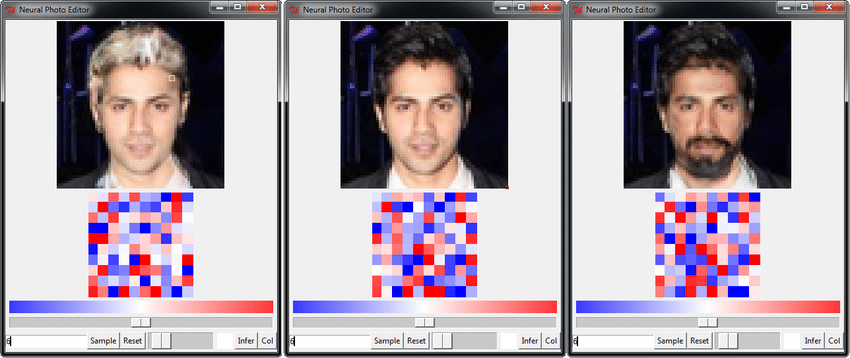
\includegraphics[width=4in]{NPE}
      \caption{Efekt działania Neural Photo Editor}
      \label{fig:npe}
    \end{figure}

    Skuteczność NPE (Neural Photo Editor) polega na zastosowaniu IAN
    (ang. Introspective Adversarial Network), czyli sieci złożonej z połączonych
    VAE (ang. Variational Autoencoder) oraz GAN, w taki sposób, żę dekodująca
    sieć autoenkodera jest używana jako sieć generująca w GAN.
    Poprzez przechwytywanie przez model dalekosiężnych zależności, wykorzystanie
    bloku obliczeniowego bazującego na rozszerzonych splotach o
    współdzielonych wagach oraz dzięki zastosowaniu ulepszonej generalizacji,
    udało się osiągnąć dokładną rekonstrukcje obrazu bez strat na jakości detali.


  \subsection{TRANSFORMING PHOTOS TO COMICS USING CONVOLUTIONAL NEURAL NETWORKS}

  \subsection{Coloring black and white world using Deep Neural Nets}

  \subsection{A Neural Algorithm of Artistic Style}

  \subsection{Face App}
